\documentclass{standalone}
\usepackage{comment}
\usepackage{tikz}
\usepackage{curves}
\usepackage{pgfplots}
\usepackage{chemfig}
%new style chemfig settings
\setchemfig{angle increment=30,atom sep=2.75em}
%deprecated chemfig settings (use if above throws error)
%\setangleincrement{30}
%\setatomsep{2.75em} %3em is default value

\pgfplotsset{compat=1.13}

%N.B. I once wrote little functions where I could define and adjust spacing with variables
%Because these figures aren't that big and it's nice to be able to make little changes,
%I stopped doing that
%Instead, all the relevant coordinates are defined here and turned into variables
%Then we draw lines to connect the variables and can make manual adjustments to the lines

%column locations (x coords)
\newcommand\Rx{0.0} %lines start here (reactant)
\newcommand\Px{12.0} %lines end here (product)
\newcommand\honohx{4.0} %Well 1
\newcommand\honhox{8.0} % Well 2
\newcommand\tsAx{2.0} % Barrier 1
\newcommand\tsBx{6.0} % Barrier 2
\newcommand\tsCx{10.0} % Barrier 3
\newcommand\Lx{13.4} %labels end here

%can define vars for energy levels (y coords)
\newcommand\Ehandhnoo{0.86}
\newcommand\Ehandcishono{-0.03}%was 0.00, but now lump cis and trans
\newcommand\Ehandtranshono{-0.03}
\newcommand\Ehonoh{-3.43}
\newcommand\Ehonho{-3.19}
\newcommand\Eohandhno{0.03}
\newcommand\Enoandhho{-6.82}
\newcommand\Ehhandnoo{-2.54}

%Energy (y-axis) limits
\newcommand\ymax{2}
\newcommand\ymin{-7}

\begin{document}
%\definecolor{gray}{gray}{0.1}
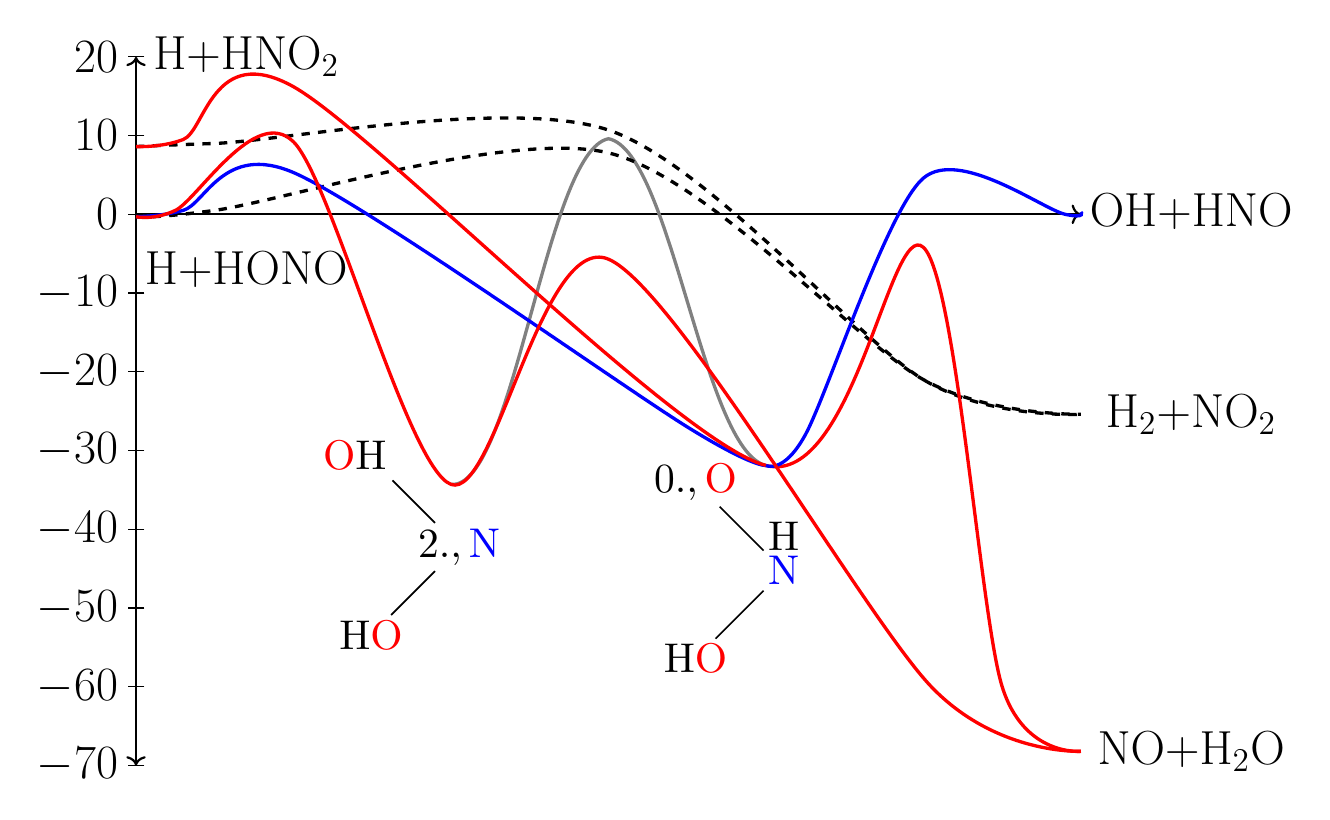
\begin{tikzpicture}%[yscale = 0.75]
%draw coordinate axis with labels
%as above, not so many label, so they are manual here (e.g. make log)
    \draw[->,thick] (0,0) -- coordinate (x axis mid) (\Px,0);
    \draw[<->,thick] (0,\ymax) -- coordinate (y axis mid)(0,\ymin);
    %\draw[gray, dashed](0,\ymax) grid (\Px,\ymin);
    \foreach \y/\ytext in {2/20,1/10,0/0,-1/-10,-2/-20,-3/-30/,-4/-40,-5/-50,-6/-60,-7/-70}%,-6/-60,-7/-70,-8/-80,-9/-90,-10/-100,-11/-110,-12/-120,-13/-130
        \draw (3pt,\y cm) -- (-3pt,\y cm) node[anchor=east] {\LARGE{$\ytext$}};

%Text Labels
%reactant side: placement will need to be adjusted for path lines
\node [scale = 1.0,black] at (1.4, 2.0){\LARGE{H+HNO$_2$}};
%\node [scale = 1.0,blue]  at (1.1,-0.3){H+cisHONO};
\node [scale = 1.0,black]   at (1.4,-0.7){\LARGE{H+HONO}}; %was transHONO (red)       
%product side: locations shouldn't need adjustment from variables, above        
\node [scale = 1.0,black] at (\Lx,\Eohandhno) {\LARGE{OH+HNO}};
\node [scale = 1.0,black] at (\Lx,\Enoandhho) {\LARGE{NO+H$_2$O}};
\node [scale = 1.0,black] at (\Lx,\Ehhandnoo) {\LARGE{H$_2$+NO$_2$}};

%Structure Labels
%\node [scale = 1.0,black] at (\honhox,-5.5) {\chemfig{H{\color{red}O}-[0]{\color{blue}N}H(-[2,,1,] \lewis{2.,{\color{red}O}})}};
\node [scale = 1.5,black] at (3.5,-4.2) {\chemfig{H{\color{red}O}-[1]{\lewis{2.,\color{blue}N}}-[11]{\color{red}O}H}};
\node [scale = 1.5,black] at (7.5,-4.5) {\chemfig{H{\color{red}O}-[1]\chemabove{{\color{blue}N}}{H}(-[11] \lewis{0.,{\color{red}O}})}};
%\draw[->,thick] (\honhox,-4.0) --(\honhox,-3.3);
   
%draw paths: nodes through which line passes (bimolecular, well, barrier)
%below are both standard draw with major points and intermediate control points
%and plot [smooth] (same arguments, different syntax)
%
%quick start: draw all your connections as (style, color, thickness up to you):
%\draw[dashed, black, very thick] plot [smooth] coordinates {(\Rx,\Ehandcishono)(\tsBx,0.78)(\Px,\Ehhandnoo)};
%add control coordinate pairs between the major coordinates to curve the lines to look good
%
%These will be layered, so the first entry is at the background
%You can fully specify each possible pathway as a line to turn some on and off,
%but it is hard to make them cleanly overlay each other
%Better is to start with full paths, decide how to layer the lines (back to front)
%and then comment out or remove the pieces of lines that aren't nicely overlaid
 
%link wells
 \draw[gray, very thick] (\honohx,\Ehonoh)..controls(4.8,-3.5)and(5.2,0.8) ..(\tsBx,0.96) ..controls(6.8,0.8)and(7.2,-3.0) ..(\honhox,\Ehonho);  
%do double well first in background 
  %H+c/tHONO=HONOH=HONHO=OH+HNO/NO+H2O
%\draw[dashed, green, very thick] plot [smooth] coordinates {(\Rx,\Ehandcishono)   (\tsAx,0.96) (\honohx,\Ehonoh) (\tsBx,0.96)  (\honhox,\Ehonho) (\tsCx,0.00) (\Px,\Eohandhno)};
%\draw[green, very thick] plot [smooth] coordinates  {(\Rx,\Ehandtranshono) (\tsAx,0.92) (\honohx,\Ehonoh) (\tsBx,0.96)  (\honhox,\Ehonho) (\tsCx,0.00) (\Px,\Eohandhno)};  
%\draw[dashed, orange, very thick] plot [smooth] coordinates {(\Rx,\Ehandcishono)   (\tsAx,0.96) (\honohx,\Ehonoh) (\tsBx,0.96)  (\honhox,\Ehonho) (\tsCx,-0.42) (\Px,\Enoandhho)};
%\draw[orange, very thick] plot [smooth] coordinates  {(\Rx,\Ehandtranshono) (\tsAx,0.92) (\honohx,\Ehonoh) (\tsBx,0.96)  (\honhox,\Ehonho) (\tsCx,-0.42) (\Px,\Enoandhho)}; 
 
  %H+{HONO}=H2+NO2
 \draw[dashed, black, very thick] plot [smooth] coordinates {(\Rx,\Ehandcishono)(1.0,0.05)(\tsBx,0.78)(10.0,-2.1)(\Px,\Ehhandnoo)};
% \draw[red, very thick] plot [smooth] coordinates {(\Rx,\Ehandtranshono)(1.0,0.1)(\tsBx,1.55)(10.0,-2.1)(\Px,\Ehhandnoo)}; 
 \draw[dashed, black, very thick] plot [smooth] coordinates {(\Rx,\Ehandhnoo)(1.0,0.9)(\tsBx,1.07)(10.0,-2.1)(\Px,\Ehhandnoo)};

  %H+{HONO}=HONHO=NO+H2O
  %cis complete path, trans, hno2 to first well
% \draw[dashed, blue, very thick] plot [smooth] coordinates {(\Rx,\Ehandcishono)  (0.6,0.1) (\tsAx,0.56) (\honhox,\Ehonho) (\tsCx,-0.42) (11.0,-6.0) (\Px,\Enoandhho)}; % 
 \draw[blue, very thick] plot [smooth] coordinates  {(\Rx,\Ehandtranshono)(0.6,0.05) (\tsAx,0.53) (7.0,-2.7) (\honhox,\Ehonho)}; %(5.0,-1.45)(7.0,-2.75)
 \draw[red, very thick] plot [smooth] coordinates       {(\Rx,\Ehandhnoo)     (0.6,0.95) (\tsAx,1.62)(\honhox,\Ehonho)(\tsCx,-0.42) (11.0,-6.0) (\Px,\Enoandhho)}; 
 
 
  %H+{HONO}=HONHO=OH+HNO
  %only need well to product for all isomers
% \draw[blue, very thick] (\honhox,\Ehonho) ..controls(9.0,-3.3)and(11.0,0.0) ..(\Px,\Eohandhno); %(\Rx,\Ehandcishono)   (\tsAx,0.56) 
 \draw[blue, very thick] plot [smooth] coordinates {(\honhox,\Ehonho) (8.5,-2.8) (\tsCx, 0.46) (11.8, 0.0) (\Px,\Eohandhno)};
 % \draw[blue, very thick] plot [smooth] coordinates  {(\Rx,\Ehandtranshono)(0.6,0.05) (\tsAx,0.53)(\honhox,\Ehonho)(\Px,\Eohandhno)};
% \draw[red, very thick] plot [smooth] coordinates  {(\Rx,\Ehandtranshono) (\tsAx,0.53) (\honhox,\Ehonho)(\Px,\Eohandhno)}; 
% \draw[very thick] plot [smooth] coordinates       {(\Rx,\Ehandhnoo)      (\tsAx,1.62) (\honhox,\Ehonho)(\Px,\Eohandhno)};  

 %alt: combine OH path with linked wells
%  \draw[green, very thick]  plot [smooth] coordinates {(\honohx,\Ehonoh)(4.8,-2.8)(\tsBx,0.96)(\honhox,\Ehonho)(11.0,-0.3)(\Px,\Eohandhno)};

  %H+c/tHONO=HONOH=NO+H2O
  %cis complete path, trans to first well
% \draw[dotted, blue, very thick] plot [smooth] coordinates {(\Rx,\Ehandcishono)(0.5,0.1)(\tsAx,0.96)(\honohx,\Ehonoh) (\tsBx,-0.57) (10.1,-6.0) (\Px,\Enoandhho)}; %
 \draw[red, very thick] plot [smooth] coordinates  {(\Rx,\Ehandtranshono)(0.5,0.05)(\tsAx,0.92)(\honohx,\Ehonoh) (\tsBx,-0.57) (10.1,-6.0) (\Px,\Enoandhho)};%(3.2,-1.9)(3.75,-3.2)



\end{tikzpicture}
% \\
% \chemfig{=\lewis{2.,C}-[:-30]\ch{+ O2}}



\end{document}
